% !TEX root = ./../../../_Thesis.tex

\begin{figure*}[h]
	\centering

	\begin{tabular}{@{}r@{ } c@{ } c@{ } c@{ } c@{ } c }
	&
	\small{Input Letter} &
	\small{Aberrated Wavefront} &
	\small{Spatial PSF} &
	\small{Simulation} & \\ \\

	\begin{sideways} \parbox[b]{25mm} {} \end{sideways} &
	
\includegraphics[width= 0.22\textwidth]{__Images/05/synthetic_sims/C_20-200@4x.png} &
	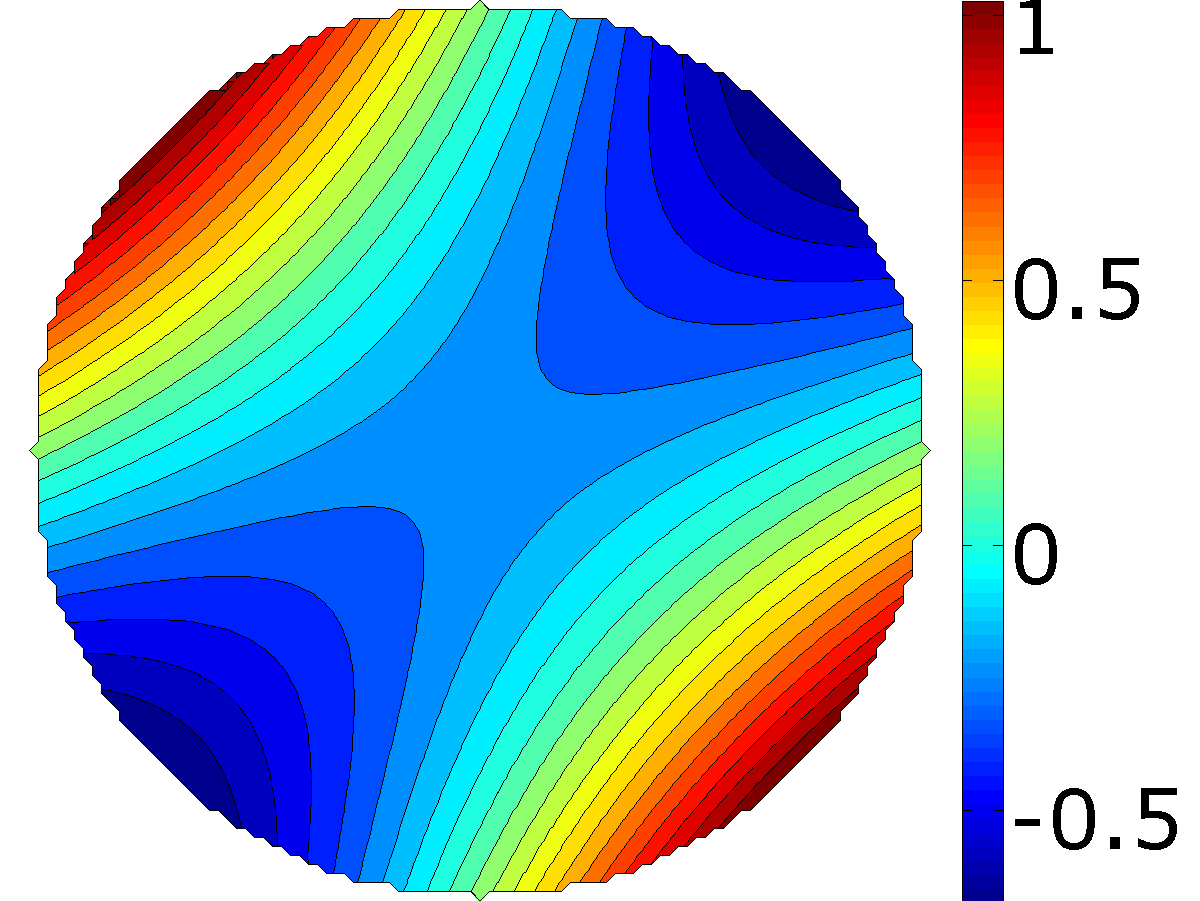
\includegraphics[height=0.22\textwidth]{__Images/05/synthetic_sims/Wavefront_0,5D,-2@45.png} &
	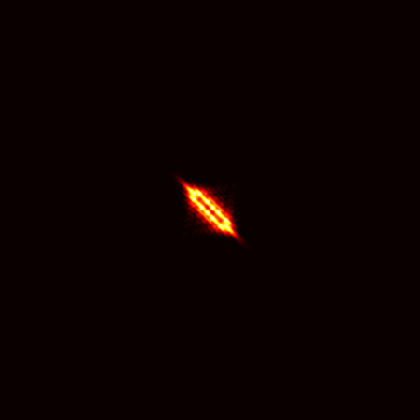
\includegraphics[width= 0.22\textwidth]{__Images/05/synthetic_sims/PSF_0,5D,-2@45.png} &
	
\includegraphics[width= 0.22\textwidth]{__Images/05/synthetic_sims/C_20-200_f50_simulated(0,5D,-2@45).png} 			\\ \\

	\begin{sideways} \parbox[b]{25mm} {} \end{sideways} &
	
\includegraphics[width= 0.22\textwidth]{__Images/05/synthetic_sims/O_20-200@4x.png} &
	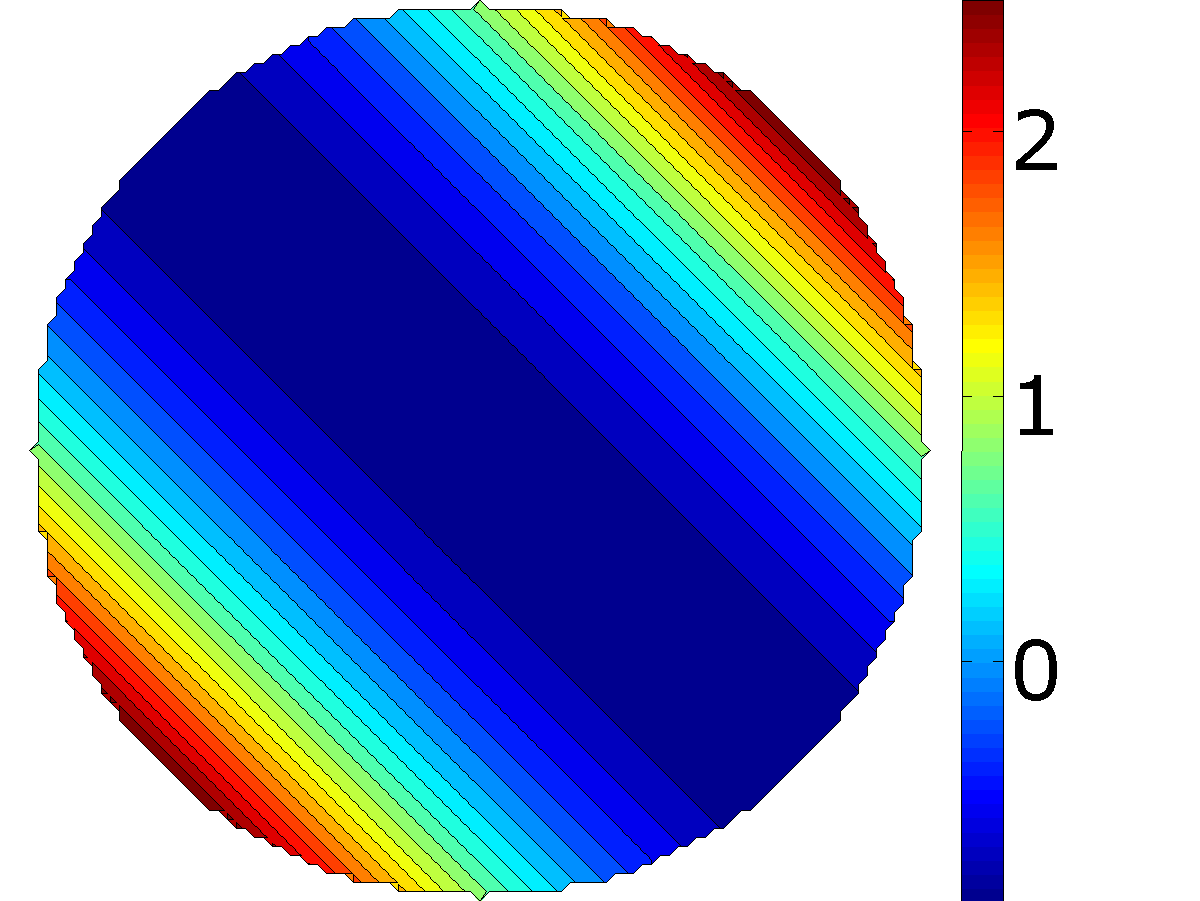
\includegraphics[height=0.22\textwidth]{__Images/05/synthetic_sims/Wavefront_0D,-4,7@135.png} &
	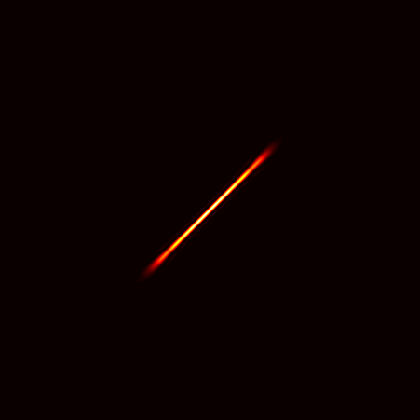
\includegraphics[width= 0.22\textwidth]{__Images/05/synthetic_sims/PSF_0D,-4,7@135.png} &
	
\includegraphics[width= 0.22\textwidth]{__Images/05/synthetic_sims/O_20-200_f50_simulated(0D,-4,7@135).png}			\\ \\

	\begin{sideways} \parbox[b]{25mm} {} \end{sideways} &
	
\includegraphics[width= 0.22\textwidth]{__Images/05/synthetic_sims/R_20-200@4x.png} &
	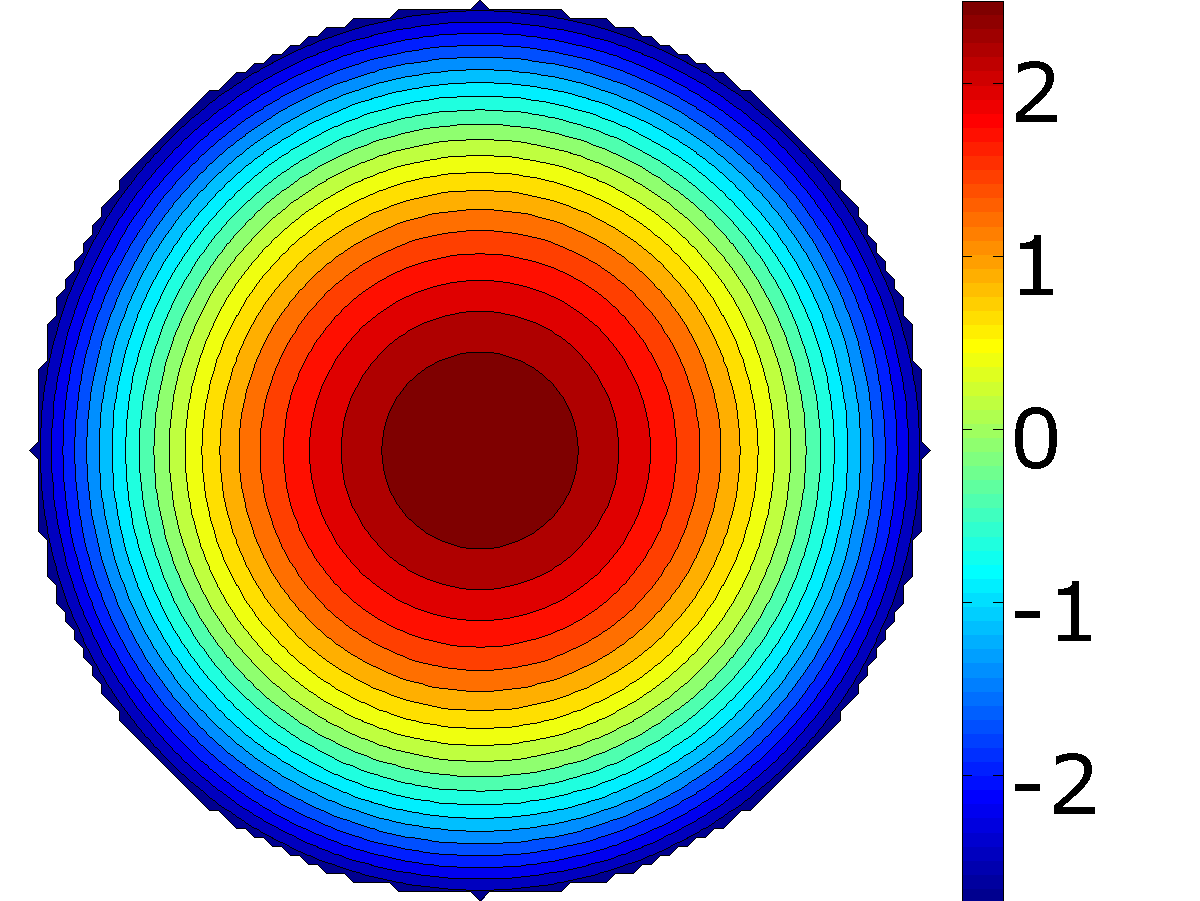
\includegraphics[height=0.22\textwidth]{__Images/05/synthetic_sims/Wavefront_6D,0@0.png} &
	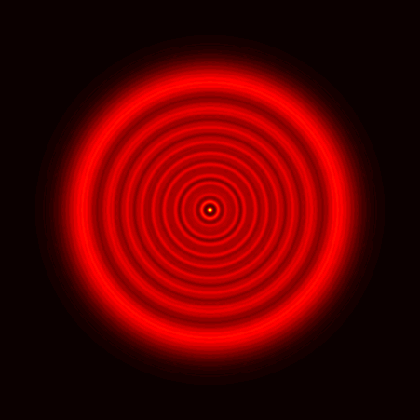
\includegraphics[width= 0.22\textwidth]{__Images/05/synthetic_sims/PSF_6D,0@0.png} &
	
\includegraphics[width= 0.22\textwidth]{__Images/05/synthetic_sims/R_20-200_f50_simulated(6D,0@0).png}				\\ \\
	
	\begin{sideways} \parbox[b]{25mm} {} \end{sideways} &
	
\includegraphics[width= 0.22\textwidth]{__Images/05/synthetic_sims/S_20-200@4x.png} &
	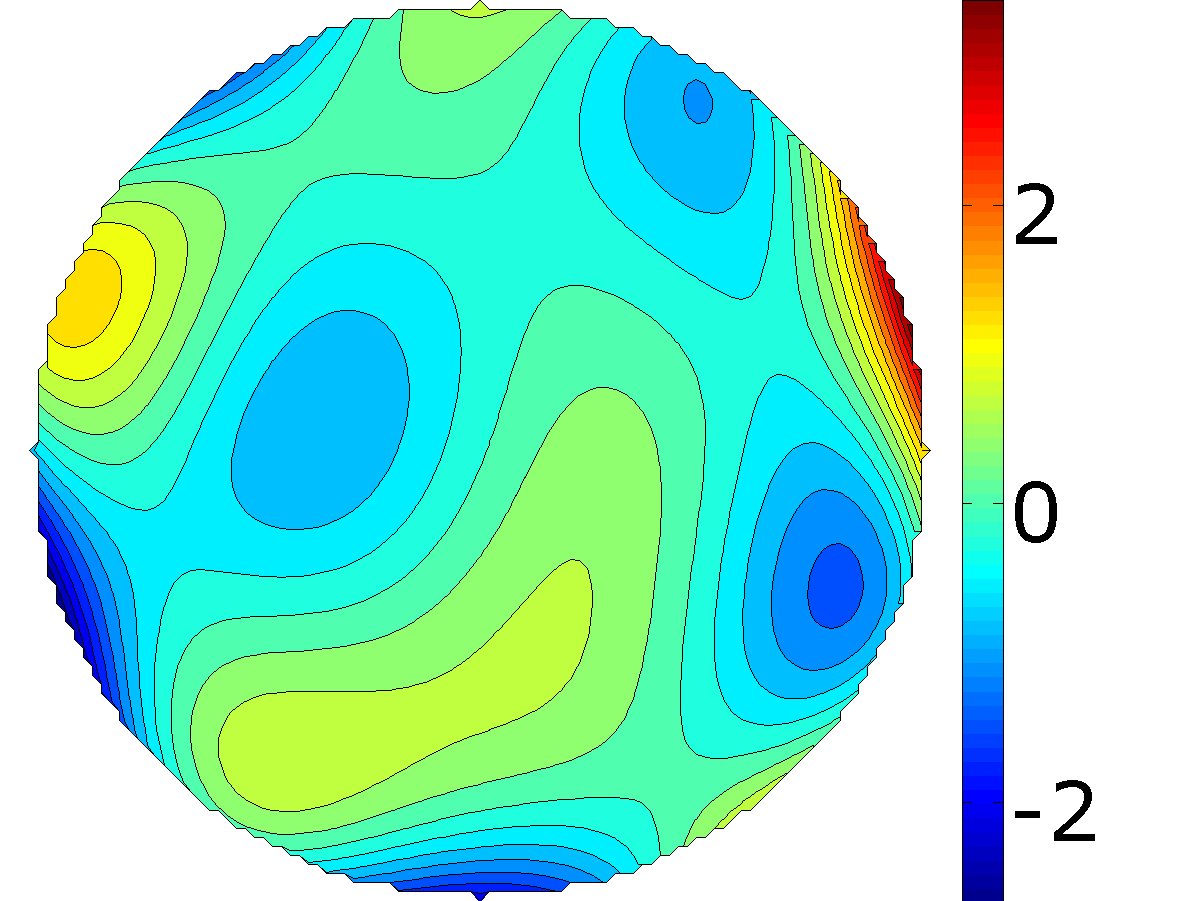
\includegraphics[height=0.22\textwidth]{__Images/05/synthetic_sims/Wavefront_highorder.png} &
	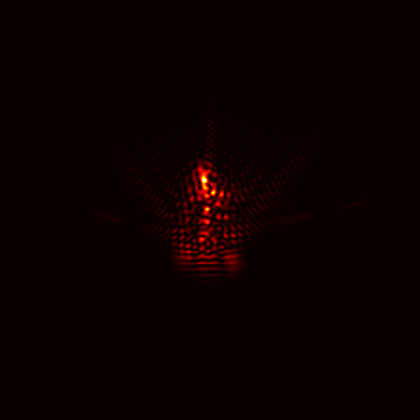
\includegraphics[width= 0.22\textwidth]{__Images/05/synthetic_sims/PSF_highorder.png} &
	
\includegraphics[width= 0.22\textwidth]{__Images/05/synthetic_sims/S_20-200_f50_simulated(high-order).png}			\\

	\end{tabular}
	
	\caption[Simulations with arbitrary wavefronts]{Simulations with arbitrary wavefronts. The input letter images correspond to a Snellen ratio of 20/200. (second column) Normalized aberrated wavefront. (third column) The spatial PSF. (fourth column) Our simulation results given the images shown in column \emph{Input Letter}. The top row shows how a combination of low-order aberrations (+0.5 Sph. -2.0 Cyl. at 45$^{\circ}$) affects the perception of a Sloan letter. The second and third rows simulate, respectively, higher values of pure astigmatism and spherical aberration (-4.7 Cyl. at 135$^{\circ}$ and +6 Sph.) than one can capture with the lenses available in our trial lens set. The bottom row shows the results of a simulation involving only higher-order aberrations ($Z^{-3}_{3}=0.2$, $Z^{-1}_{3}=0.2$, $Z^{3}_{3}=0.1$, $Z^{2}_{4}=0.2$, $Z^{-5}_{5}=0.4$, $Z^{1}_{5}=0.3$).}
	\label{fig:synthetic_sims}
\end{figure*}

\clearpage
